\documentclass[10pt]{article}
\usepackage[margin=0.5in, top=0.4in, bottom=0.5in]{geometry}
\usepackage{graphicx}
\usepackage{xcolor}
\usepackage{fontspec}
\usepackage{hyperref}
\usepackage{parskip}
\usepackage{multicol}
\usepackage{fancyhdr}

% Colors
\definecolor{muted}{HTML}{555555}
\definecolor{accent}{HTML}{e85d75}

% Typography
\setmainfont{Helvetica Neue}[
  UprightFont = *,
  BoldFont = * Bold,
  ItalicFont = * Italic,
]

% Hyperlinks
\hypersetup{
  colorlinks=true,
  linkcolor=accent,
  urlcolor=accent,
  pdfauthor={Nathan Turczan},
  pdftitle={Nathan Turczan - Portfolio},
}

% Page style
\pagestyle{fancy}
\fancyhf{}
\renewcommand{\headrulewidth}{0pt}
\fancyfoot[R]{\footnotesize\color{muted} nathanturczan.com}

% Reduce paragraph spacing
\setlength{\parskip}{0.4em}

% Custom commands
\newcommand{\sectionline}{\vspace{0.3em}\hrule\vspace{0.6em}}

\newcommand{\projectentry}[6]{%
  \noindent
  \begin{minipage}[t]{0.24\textwidth}
    \vspace{0pt}
    \href{#6}{\includegraphics[width=\textwidth]{#1}}
  \end{minipage}%
  \hfill%
  \begin{minipage}[t]{0.73\textwidth}
    \vspace{0pt}
    {\normalsize\bfseries \href{#6}{#2}} \hfill {\scriptsize\color{muted} #3}

    \vspace{0.2em}
    {\scriptsize\color{muted}\textbf{PROBLEM:}} {\scriptsize #4}

    \vspace{0.15em}
    {\scriptsize\color{muted}\textbf{BUILT:}} {\scriptsize #5}
  \end{minipage}
  \vspace{0.9em}
}

\begin{document}

% === HERO PAGE ===
\thispagestyle{empty}

\begin{center}
{\LARGE\bfseries NATHAN TURCZAN}

\vspace{0.15em}
{\normalsize Composer / Product Designer / Creative Technologist}

\vspace{0.1em}
{\scriptsize\color{muted} Los Angeles \quad · \quad nathanturczan@gmail.com \quad · \quad nathanturczan.com}
\end{center}

\vspace{0.6em}

% Hero image - Scale Navigator Dashboard
\begin{center}
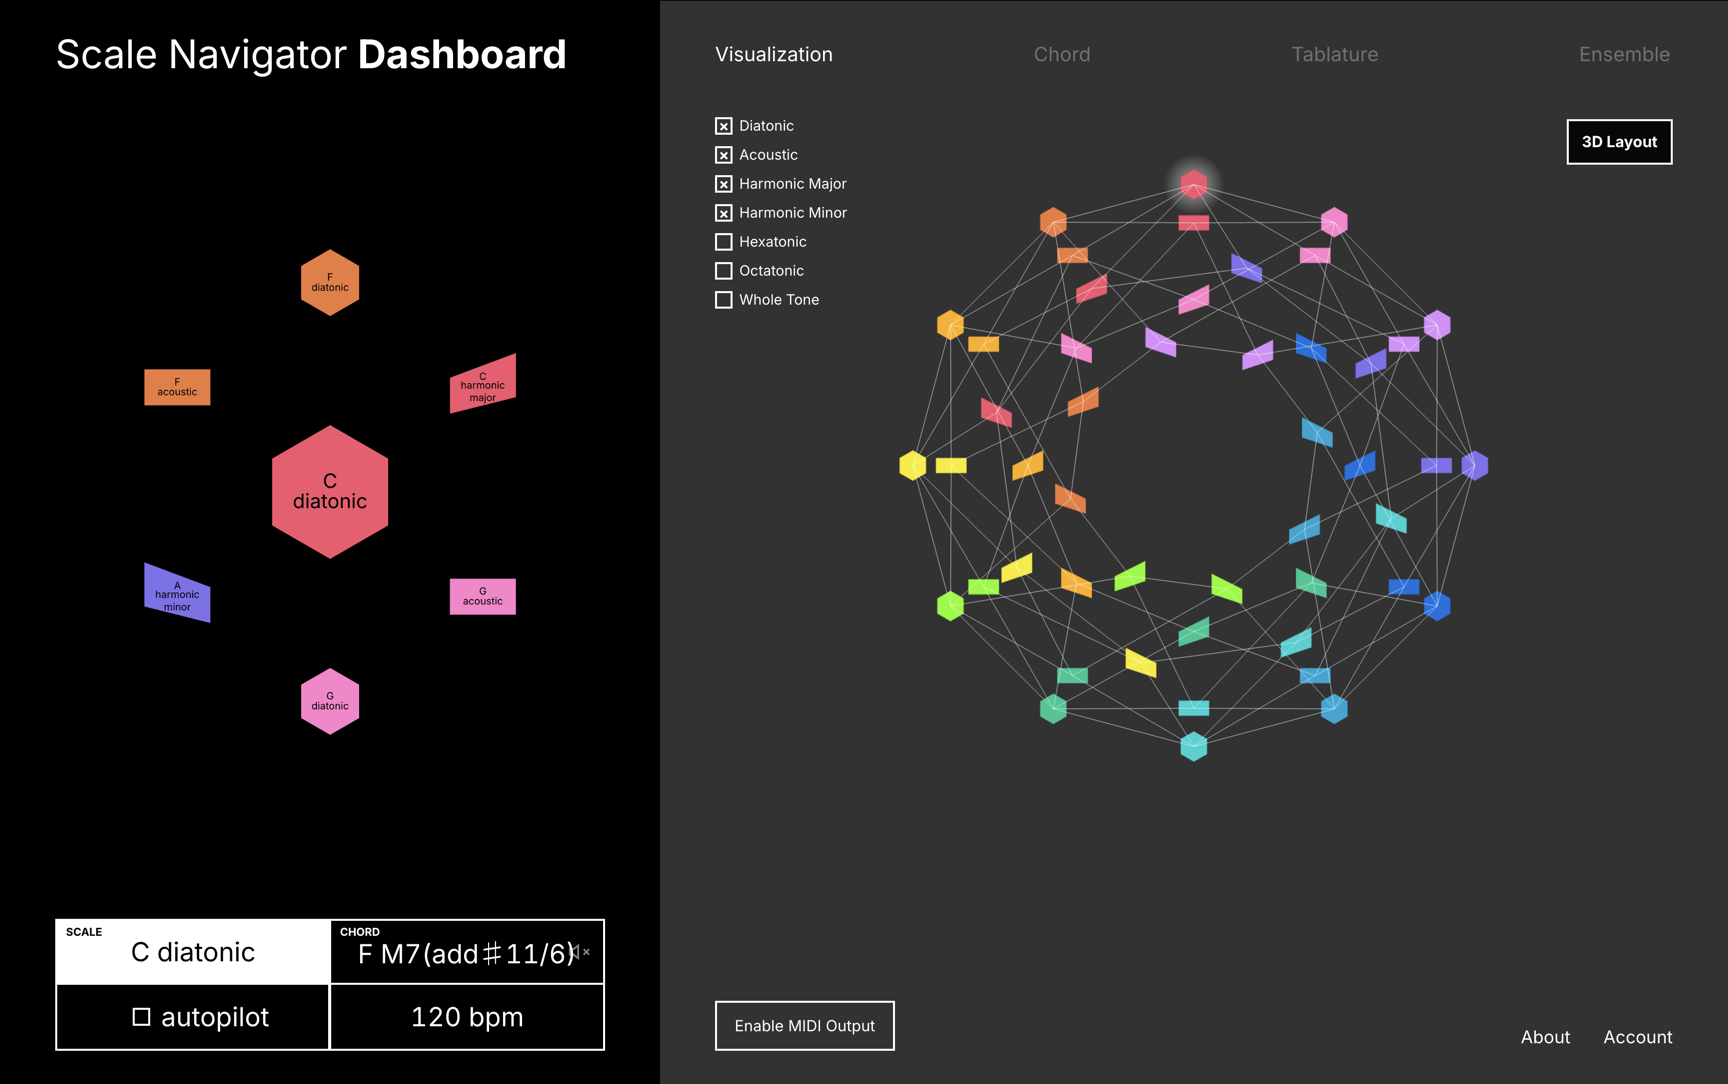
\includegraphics[width=\textwidth]{images/dashboard/scalenavigatordashboard.png}
\end{center}

\vspace{0.3em}

\begin{center}
{\normalsize\itshape Building instruments that let people navigate harmony as interactive space.}
\end{center}

\vspace{0.5em}

{\small I design and build software instruments that transform abstract music theory into navigable, playable environments. My work spans DAW plugins, web applications, mobile apps, networked performance systems, and interactive installations.

Currently developing the \textbf{Scale Navigator} ecosystem: harmonic middleware that coordinates your entire session from one interface. The visualization above maps 57 scales into a network where adjacent nodes differ by a single note, enabling smooth voice leading between any two harmonic states.}

\sectionline

% === SELECTED PROJECTS ===

{\large\bfseries SELECTED PROJECTS}
\vspace{0.6em}

% Project 1: Scale Navigator Dashboard
\projectentry{images/dashboard/desktop/Screenshot 2026-02-17 at 9.26.07 AM.png}
{Scale Navigator Dashboard}
{2021–Present}
{Producers lack a unified way to coordinate harmony across DAW, plugins, and instruments. Scale changes require manual updates to multiple tools.}
{Cross-platform harmonic middleware (Web, iOS, Android, VST3/AU) that broadcasts scale and chord state via MIDI. One source of truth for your session's harmony. Free on all platforms.}
{https://scalenavigator.com}

% Project 2: LA Laptop Orchestra
\projectentry{images/lalork/poster-1.jpg}
{LA Laptop Orchestra}
{2026}
{Experimental music communities lack accessible entry points. Laptop orchestras historically require technical expertise, excluding casual participants.}
{Participatory public music ritual where strangers join a shared harmonic field via QR code. Phones, laptops, and acoustic instruments all connect to the same harmony: no wrong notes possible. Launching August 2026 at Scribble, Los Angeles.}
{https://lalaptoporchestra.com}

% Project 3: Tonalign
\projectentry{images/tonalign/tonalign-1.png}
{Tonalign}
{2024–Present}
{MIDI pitch correction tools don't exist. Producers can autotune vocals but not MIDI: they must manually correct notes outside the current scale.}
{Polyphonic MIDI pitch correction plugin (VST3/AU). Routes incoming notes to nearest scale degree in real time. Try chord ideas in any scale: hear what works instantly.}
{https://scalenavigator.com}

% Project 4: SOULS
\projectentry{images/souls-main.jpg}
{SOULS (with Sia \& David O'Reilly)}
{2022}
{Interactive NFT characters needed ambient soundscapes that felt alive and responsive, not static audio loops.}
{Procedural audio system generating unique ambient compositions for 10,000 collectible characters. Each SOUL has its own evolving sonic identity. Featured in Forbes, Designboom, OpenSea.}
{https://opensea.io/collection/souls-of-nature}

% Project 5: Modal Intersections
\projectentry{images/modal.png}
{Modal Intersections}
{2018}
{Audiences experience generative music passively. Interactive installations rarely give meaningful musical control to untrained participants.}
{Audiovisual installation where audience movement controls real-time harmonic transitions. Player pianos respond to gesture; projections visualize shifting modal relationships. Exhibited at CalArts CEAIT Festival and REDCAT Gallery.}
{https://nathanturczan.com/projects/modal-intersections.html}

% Project 6: Ensemble Jammer
\projectentry{images/ensemblejammer/Screenshot 2026-02-17 at 6.32.10 PM.png}
{Ensemble Jammer}
{2024–Present}
{Remote musicians can't improvise together without latency issues and harmonic chaos.}
{Networked instrument app (Web, iOS) where host controls harmony, players respond with constrained instruments: Touch Harp, Drone, Sequencer. Firebase real-time sync. No wrong notes. Used for sound baths and remote jams.}
{https://ensemblejammer.scalenavigator.com}

\sectionline

% === ADDITIONAL WORK ===
{\large\bfseries ADDITIONAL WORK}
\vspace{0.4em}

\begin{multicols}{2}
\noindent{\small\bfseries \href{https://nathanturczan.com/projects/snaps-plugin.html}{SNaPS Plugin}} {\scriptsize\color{muted} 2024 · Sampler/VST3}\\
{\scriptsize Harmony-aware granular sampling with 8 particle emitters. Co-developed with Nathan Ho.}

\vspace{0.5em}
\noindent{\small\bfseries \href{https://early-downhome-blues.scalenavigator.com}{Early Downhome Blues}} {\scriptsize\color{muted} 2024 · Web}\\
{\scriptsize Interactive blues melody generator based on Jeff Todd Titon's musicology research.}

\vspace{0.5em}
\noindent{\small\bfseries \href{https://nathanturczan.com/projects/pandiatonic-autoharp.html}{Pandiatonic Autoharp}} {\scriptsize\color{muted} 2021 · Instrument}\\
{\scriptsize Modified autoharp retuned for pandiatonic exploration: all seven diatonic notes.}

\columnbreak

\noindent{\small\bfseries \href{https://nathanturczan.bandcamp.com/album/to-a-wild-rose-growing-throughout-the-multiverse}{To A Wild Rose...}} {\scriptsize\color{muted} 2020 · Album}\\
{\scriptsize 14 algorithmic remixes of Edward MacDowell via sample rate modulation.}

\vspace{0.5em}
\noindent{\small\bfseries \href{https://scalenavigator.com}{Scale Awareness Bridge}} {\scriptsize\color{muted} 2024 · M4L}\\
{\scriptsize Syncs Scale Navigator to Ableton's native scale mode and Push.}

\vspace{0.5em}
\noindent{\small\bfseries \href{https://scalenavigator.com}{Voice Leader}} {\scriptsize\color{muted} 2023 · M4L}\\
{\scriptsize Four-voice SATB harmony from single notes, based on Huron's Bach/Haydn analysis.}
\end{multicols}

\sectionline

% === BACKGROUND & SKILLS ===
\noindent
\begin{minipage}[t]{0.48\textwidth}
{\normalsize\bfseries BACKGROUND}
\vspace{0.3em}

{\scriptsize
\textbf{MFA Music Technology} — CalArts, 2018

\textbf{BA Vocal Performance} — UC Santa Cruz, 2013

Thesis: Scale Navigator interface design based on Dmitri Tymoczko's voice-leading geometry research (NIME 2019 paper).

CTO and Co-founder, Chordas Collective (choral tech).
}
\end{minipage}%
\hfill%
\begin{minipage}[t]{0.48\textwidth}
{\normalsize\bfseries SKILLS}
\vspace{0.3em}

{\scriptsize
\textbf{Languages:} JavaScript/TypeScript, C++, Python, Max/MSP, SuperCollider

\textbf{Frameworks:} React, JUCE, Tone.js, Firebase, Capacitor

\textbf{Tools:} Ableton Live, Figma, Git, LaTeX, LilyPond

\textbf{Domains:} Audio plugin dev, real-time web audio, MIR, networked performance, interactive installation
}
\end{minipage}

\vspace{1em}

\begin{center}
{\normalsize\color{muted} — }

\vspace{0.3em}
{\small Available for creative technology roles, interactive sound design, and music technology consulting.}

\vspace{0.2em}
{\small\bfseries nathanturczan@gmail.com \quad · \quad nathanturczan.com \quad · \quad github.com/nathanturczan}
\end{center}

\end{document}
